\documentclass[handout]{beamer}

\usetheme[progressbar=frametitle]{metropolis}
\usepackage{appendixnumberbeamer}
\usepackage{booktabs}
\usepackage{amsmath}
\usepackage{amssymb}
\usepackage{tcolorbox}
\usepackage{tikz}
\usetikzlibrary{bayesnet}
\definecolor{metropolisblue}{RGB}{39, 59, 94}



% Begin document
\begin{document}


% Title page
\title{Maximum Likelihood Estimation}
\author{Nipun Batra}
\date{\today}
\institute{IIT Gandhinagar}
\maketitle
\setbeamercovered{invisible}
\begin{frame}
    \frametitle{Agenda}
    \tableofcontents[hidesubsections]
    \end{frame}
    
\begin{section}{Revision - Prior, Posterior, MLE, MAP}
\end{section}
\begin{section}{Distributions, IID}
    \begin{frame}
        Notebook
    \end{frame}

    \begin{frame}{Graphical model}
        Assume model parameters are $\theta$ and data is $D  $. We can write the joint probability distribution as:

        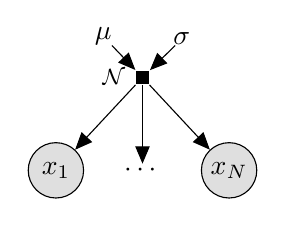
\begin{tikzpicture}
            \node[obs] (x1) {$x_1$};
            \node[const, right=0.5cm of x1]                               (dots) {$\cdots$};
            \node[obs, right=0.5cm of dots]                               (xn) {$x_N$};
            
            \factor[above=1 of dots] {y-f} {left:${\mathcal{N}}$} {} {} ; %
            \node[const, above=1.5 of dots, xshift=0.5cm] (sigma) {$\mathbf{\sigma}$};
            \node[const, above=1.5 of dots, xshift=-0.5cm] (mu) {$\mathbf{\mu}$};
            \edge {y-f} {dots} ;
            \edge {y-f} {xn} ; %
            \edge {y-f} {x1} ;
            \edge {mu, sigma} {y-f} ; %           
            
        \end{tikzpicture}
        
    \end{frame}

    \begin{frame}{Graphical model}
        Assume model parameters are $\theta$ and data is $D  $. We can write the joint probability distribution as:

        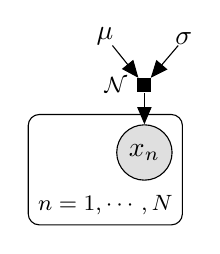
\begin{tikzpicture}
                
                
            \node[obs]                               (xn) {$x_n$};
            \factor[above=of xn] {y-f} {left:${\mathcal{N}}$} {} {} ; %
            \node[const, above=1 of xn, xshift=0.5cm] (sigma) {$\mathbf{\sigma}$};
            \node[const, above=1 of xn, xshift=-0.5cm] (mu) {$\mathbf{\mu}$};
            \plate{}{(xn)}{$n = 1, \cdots, N$};
            
            
            
            \edge {y-f} {xn} ; %
            \edge {mu, sigma} {y-f} ; %
            
            
        \end{tikzpicture}
        
    \end{frame}

    \begin{frame}{Factorisation}
        \begin{align*}
            P(D|\theta) & = P(x_1, x_2, \ldots, x_n | \theta) \\
            & = P(x_1|\theta) \cdot P(x_2|\theta) \cdot \ldots \cdot P(x_n|\theta)
        \end{align*}
        
    \end{frame}

\end{section}

\section{MLE}
\begin{frame}{Pop Quiz}
    We have three courses: C1, C2, C3. Assume no student takes more than one course.
    The scores of students in these courses are normally distributed with the following parameters:
    \begin{itemize}
        \item C1: $\mu_1 = 80, \sigma_1 = 10$
        \item C2: $\mu_2 = 70, \sigma_2 = 10$
        \item C3: $\mu_3 = 90, \sigma_3 = 5$
    \end{itemize}


    
\end{frame}

\begin{frame}{Pop Quiz}
    We have three courses: C1, C2, C3. Assume no student takes more than one course.
    The scores of students in these courses are normally distributed with the following parameters:
    \begin{itemize}
        \item C1: $\mu_1 = 80, \sigma_1 = 10$
        \item C2: $\mu_2 = 70, \sigma_2 = 10$
        \item C3: $\mu_3 = 90, \sigma_3 = 5$
    \end{itemize}

   
    I randomly pick up a student and ask them their marks. They say 82. Which course do you think they are from?
    To keep things simple, for now assume that all three courses have equal number of students.
    
    
    
\end{frame}

\begin{frame}{Pop Quiz}
    We have three courses: C1, C2, C3. Assume no student takes more than one course.
    The scores of students in these courses are normally distributed with the following parameters:
    \begin{itemize}
        \item C1: $\mu_1 = 80, \sigma_1 = 10$
        \item C2: $\mu_2 = 70, \sigma_2 = 10$
        \item C3: $\mu_3 = 90, \sigma_3 = 5$
    \end{itemize}

   
    I randomly pick up a student and ask them their marks. They say 82. Which course do you think they are from?
    
    
    
    Most likely C1. But why?
    
\end{frame}

\begin{frame}{Pop Quiz}
    Let us plot the probability density functions of the three courses. 
    \begin{figure}
        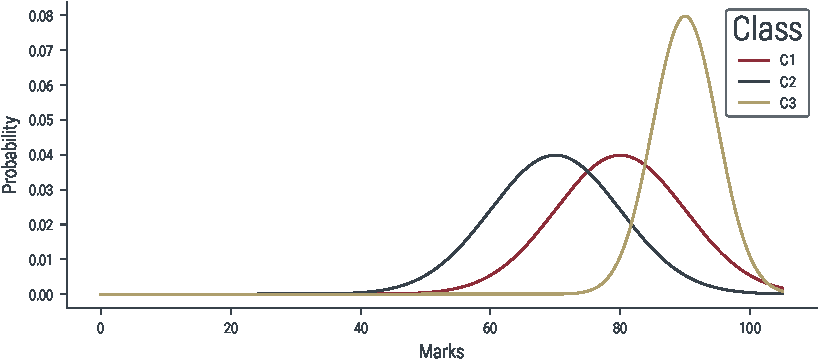
\includegraphics[width=\textwidth]{../figures/mle/mle-example.pdf}
    \end{figure}
    
\end{frame}

\begin{frame}{Pop Quiz}
    Let us plot the probability density functions of the three courses. 
    \begin{figure}
        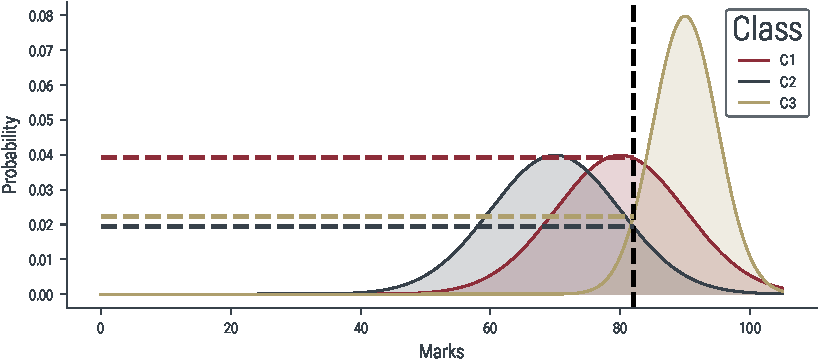
\includegraphics[width=\textwidth]{../figures/mle/mle-example-2.pdf}
    \end{figure}
    
\end{frame}

\begin{frame}
  Notebook  
\end{frame}

\begin{frame}{Pop Quiz 2}
    Let us say we observed a value of 20. We know it came from a normal distribution with $\sigma=1$. What is the most likely value of $\mu$?
    


\end{frame}

\begin{frame}{Pop Quiz 2}
    Let us say we observed a value of 20. We know it came from a normal distribution with $\sigma=1$. What is the most likely value of $\mu$?
    
    20. But why?


\end{frame}

\begin{frame}{Pop Quiz 2}
    Let us say we observed a value of 20. We know it came from a normal distribution with $\sigma=1$. What is the most likely value of $\mu$?
    
    20. But why?

    Let us evaluate probability density function at 20 for different values of $\mu$ for $\sigma=1$, i.e., $f(x=20|\mu, \sigma=1)$.


\end{frame}

\begin{frame}{Pop Quiz 2}
    Let us say we observed a value of 20. We know it came from a normal distribution with $\sigma=1$. What is the most likely value of $\mu$?
    
    20. But why?

    Let us evaluate probability density function at 20 for different values of $\mu$ for $\sigma=1$, i.e., $f(x=20|\mu, \sigma=1)$.

    Importantly, this is a function of $\mu$ and not $x$ (which is fixed at 20).

\end{frame}

\begin{frame}
    Notebook
\end{frame}

\begin{frame}{Pop Quiz 3}


Let us now go back to our original problem. We have three courses: C1, C2, C3. Assume no student takes more than one course.

We ask two students their marks. The first student says 82 and the second student says 72. Which course do you think they are from? Assumption: Both are from the same course.

Let us create a table of probabilities for each course:




    
\end{frame}
\section{MLE for Bernoulli Distribution}
\begin{frame}{MLE for Bernoulli Distribution}
The probability mass function of a bernoulli distribution is given by:

\begin{equation}
f(x|\theta) = \theta^x(1-\theta)^{(1-x)}
\end{equation}
Let us assume we have a dataset $D = \{x_1, x_2, \ldots, x_n\}$, where each $x_i$ is an independent sample from the above distribution and $x_i\in\{0, 1\}$.
We want to estimate the parameter $\theta$ from the data.
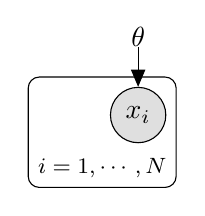
\begin{tikzpicture}
    \node[obs]                               (xi) {$x_i$};
    \node[const, above=0.5 of xi](theta)
    {$\mathbf{\theta}$};
    \plate{}{(xi)}{$i = 1, \cdots, N$};
    \edge{theta}{xi}
\end{tikzpicture}

Our likelihood function is given by:
\begin{equation}
P(D|\theta) = \mathcal{L}(\theta) = \prod_{i=1}^n f(x_i|\theta)
\end{equation}
\end{frame}

\begin{frame}{Log Likelihood Function}
    Log-likelihood function:
    \begin{equation}
        \log \mathcal{L}(\theta) = \sum_{i=1}^n \log f(x_i|\theta)
    \end{equation}

    Simplifying the above equation, we get:
    \begin{align*}
        \log \mathcal{L}(\theta) &= \sum_{i=1}^n \log f(x_i|\theta) \\
        &= \sum_{i=1}^n \log \left (\theta^{x_{i}}(1-\theta)^{(1-x_{i})} \right) \\
        &= \sum_{i=1}^n \left( \log \left( \theta^{x_{i}} \right) + \log \left( (1-\theta)^{(1-x_{i})}  \right) \right) \\
        \end{align*}
\end{frame}
\begin{frame}
   
    \begin{align*}
        \log \mathcal{L}(\theta) &= \sum_{i=1}^n \left (x_{i}\log \left( \theta \right) + (1-x_{i})\log \left(1-\theta \right) \right)\\
        \end{align*}
        \begin{tcolorbox}[colback=metropolisblue!5,colframe=metropolisblue,title=Log Likelihood Function for Bernoulli Distribution]
            Log-likelihood function for bernoulli distributed data is:
            \[
                \log \mathcal{L}(\theta) = \sum_{i=1}^n  (x_{i}\log(\theta) + (1-x_{i})\log(1-\theta))
                \]
        \end{tcolorbox}
\end{frame}

\begin{frame}
    \frametitle{Maximum Likelihood Estimate for $\theta$}
    
    To find the MLE for $\theta$, we differentiate the log-likelihood function with respect to $\theta$ and set it to zero:
    
    \begin{align*}
        \frac{\partial \log \mathcal{L}(\theta)}{\partial \theta} &= \frac{\partial}{\partial \theta} \left (\sum_{i=1}^n \left (x_{i}\log \left( \theta \right) + (1-x_{i})\log \left(1-\theta \right) \right)\right)\\
        &= \sum_{i=1}^n \left (\frac{\partial}{\partial \theta}(x_{i}\log \left( \theta \right)) + \frac{\partial}{\partial \theta}(1-x_{i})\log \left(1-\theta \right) \right)\\
        &= \sum_{i=1}^n \left (x_{i}\frac{\partial}{\partial \theta}\log \left( \theta \right) + (1-x_{i})\frac{\partial}{\partial \theta}\log \left(1-\theta \right) \right)\\
        &= \sum_{i=1}^n \left (\frac{x_{i}}{\theta} - \frac{(1-x_{i})}{1-\theta} \right)=0\\
    \end{align*}
    
    
    \end{frame}

\begin{frame}
        
    \begin{align*}
        \frac{\partial \log \mathcal{L}(\theta)}{\partial \theta} &=  \sum_{i=1}^n \left (\frac{x_{i}(1-\theta)-\theta(1-x_{i})}{\theta(1-\theta)} \right)=0\\
        &= \sum_{i=1}^n \left (\frac{x_{i}-x_{i}\theta-\theta+\theta x_{i}}{\theta(1-\theta)} \right)\\
        &= \sum_{i=1}^n \left (\frac{x_{i}-\theta}{\theta(1-\theta)} \right)\\
        &= \sum_{i=1}^n \left (x_{i}-\theta \right)=0\\
        &= \sum_{i=1}^n x_{i} - \sum_{i=1}^n\theta=0\\
        &= \sum_{i=1}^n x_{i} - n\theta=0\\
    \end{align*}
    
    
    \end{frame}

\begin{frame}
        
    \begin{align*}
        \theta=\frac{\sum_{i=1}^n x_{i}}{n}\\
    \end{align*}
    \begin{tcolorbox}[colback=metropolisblue!5,colframe=metropolisblue,title=Maximum Likelihood Estimate for $\theta$]
        MLE of $\theta$, denoted as $\hat{\theta}_{\text{MLE}}$, is given by:
        \begin{equation*}
            \hat{\theta}_{\text{MLE}} = \frac{\sum_{i=1}^n x_{i}}{n}
        \end{equation*}
    \end{tcolorbox}
    
    \end{frame}

\begin{frame}
For example if we have a Bernoulli Distribution with $\theta=0.2,$ the likelihood, $P(D|\theta)$ is given below:
\begin{figure}
                \centerline{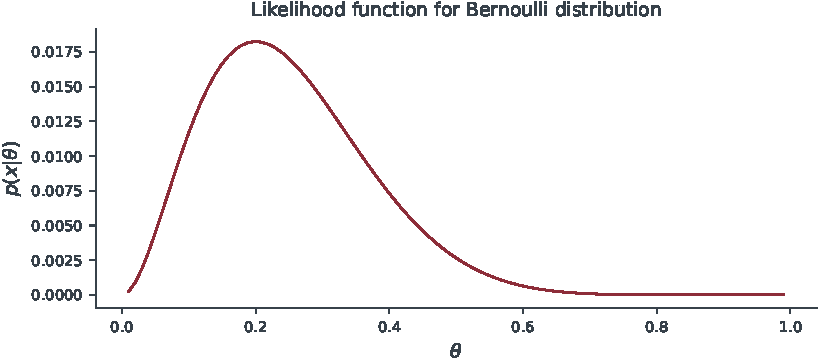
\includegraphics[scale = 0.75]{../figures/mle/bernoulli_likelihood.pdf}}
\end{figure}
    
\end{frame}



% Section 1
\section{MLE for Univariate Normal Distribution}

\begin{frame}{Univariate Normal Distribution}
The probability density function of a univariate normal distribution is given by:

\begin{equation}
f(x|\mu, \sigma^2) = \frac{1}{\sqrt{2\pi\sigma^2}}\exp\left(-\frac{(x-\mu)^2}{2\sigma^2}\right)
\end{equation}

Let us assume we have a dataset $D = \{x_1, x_2, \ldots, x_n\}$, where each $x_i$ is an independent sample from the above distribution. 
We want to estimate the parameters $\theta = \{\mu, \sigma\}$ from the data.

Our likelihood function is given by:
\begin{equation}
P(D|\theta) = \mathcal{L}(\mu, \sigma^2) = \prod_{i=1}^n f(x_i|\mu, \sigma^2)
\end{equation}


\end{frame}

\begin{frame}{Log Likelihood Function}
    Log-likelihood function:
    \begin{equation}
        \log \mathcal{L}(\mu, \sigma^2) = \sum_{i=1}^n \log f(x_i|\mu, \sigma^2)
    \end{equation}

    Simplifying the above equation, we get:
    \begin{align*}
        \log \mathcal{L}(\mu, \sigma^2) &= \sum_{i=1}^n \log f(x_i|\mu, \sigma^2) \\
        &= \sum_{i=1}^n \log \left( \frac{1}{\sqrt{2\pi\sigma^2}} \exp \left( -\frac{(x_i-\mu)^2}{2\sigma^2} \right) \right) \\
        &= \sum_{i=1}^n \left( \log \left( \frac{1}{\sqrt{2\pi\sigma^2}} \right) + \log \left( \exp \left( -\frac{(x_i-\mu)^2}{2\sigma^2} \right) \right) \right) \\
        \end{align*}
\end{frame}

\begin{frame}
   
    \begin{align*}
        \log \mathcal{L}(\mu, \sigma^2) &= \sum_{i=1}^n \left( \log \left( \frac{1}{\sqrt{2\pi\sigma^2}} \right) -\frac{(x_i-\mu)^2}{2\sigma^2} \right) \\
        &= \sum_{i=1}^n \left( -\frac{1}{2} \log (2\pi\sigma^2) -\frac{(x_i-\mu)^2}{2\sigma^2} \right) \\
        &= -\frac{n}{2} \log (2\pi\sigma^2) - \frac{1}{2\sigma^2} \sum_{i=1}^n (x_i-\mu)^2
        \end{align*}
        \begin{tcolorbox}[colback=metropolisblue!5,colframe=metropolisblue,title=Log Likelihood Function for Univariate Normal Distribution]
            Log-likelihood function for normally distributed data is:
            \[
                \log \mathcal{L}(\mu, \sigma^2) = -\frac{n}{2} \log(2\pi) - n\log(\sigma) - \frac{1}{2\sigma^2} \sum_{i=1}^n (x_i-\mu)^2
                \]
        \end{tcolorbox}
\end{frame}








\begin{frame}
    \frametitle{Maximum Likelihood Estimate for $\mu$}
    
    To find the MLE for $\mu$, we differentiate the log-likelihood function with respect to $\mu$ and set it to zero:
    
    \begin{align*}
        \frac{\partial \log \mathcal{L}(\mu, \sigma^2)}{\partial \mu} &= \frac{\partial}{\partial \mu} \left(-\frac{n}{2} \log (2\pi\sigma^2) - \frac{1}{2\sigma^2} \sum_{i=1}^n (x_i-\mu)^2\right) =0\\
        \frac{\partial}{\partial \mu} \left(\sum_{i=1}^n (x_i-\mu)^2\right) &= 0
    \end{align*}
    
    \begin{tcolorbox}[colback=metropolisblue!5,colframe=metropolisblue,title=Maximum Likelihood Estimate for $\mu$]
        MLE of $\mu$, denoted as $\hat{\mu}_{\text{MLE}}$, is given by:
        \begin{equation*}
            \hat{\mu}_{\text{MLE}} = \frac{1}{n}\sum_{i=1}^n x_i
        \end{equation*}
    \end{tcolorbox}
    
    \end{frame}

\begin{frame}{MLE for $\sigma$ for normally distributed data}
    Recall that the log-likelihood function is given by:
    \begin{equation}
        \log \mathcal{L}(\mu, \sigma^2) = \sum_{i=1}^n \log f(x_i|\mu, \sigma^2)
    \end{equation}

    Let us find the maximum likelihood estimate of $\sigma^2$ now. We can do this by taking the derivative of the log-likelihood function with respect to $\sigma^2$ and equating it to zero.   

    \begin{equation}
        \frac{\partial \log \mathcal{L}(\mu, \sigma^2)}{\partial \sigma^2} = \sum_{i=1}^n \frac{\partial \log f(x_i|\mu, \sigma^2)}{\partial \sigma^2} = 0
    \end{equation}
    
\end{frame}

\begin{frame}{MLE for $\sigma$ for normally distributed data}
    \begin{tcolorbox}[colback=metropolisblue!5,colframe=metropolisblue,title=Log Likelihood Function for Univariate Normal Distribution]
        Log-likelihood function for normally distributed data is:
        \[
            \log \mathcal{L}(\mu, \sigma^2) = -\frac{n}{2} \log(2\pi) - n\log(\sigma) - \frac{1}{2\sigma^2} \sum_{i=1}^n (x_i-\mu)^2
            \]
    \end{tcolorbox}

Now, we can differentiate the log-likelihood function with respect to $\sigma$ and equate it to zero.
\end{frame}

\begin{frame}{MLE for $\sigma$ for normally distributed data}

    
        \[
        \frac{{\partial}}{{\partial \sigma}} \log \mathcal{L}(\mu, \sigma^2) = -\frac{n}{\sigma} + \frac{1}{\sigma^3} \sum_{i=1}^n (x_i-\mu)^2 = 0
        \]
    
        Multiplying through by $\sigma^3$, we have:
    
        \[
        -n \sigma^2 + \sum_{i=1}^n (x_i-\mu)^2 = 0
        \]
    
        \begin{tcolorbox}[colback=metropolisblue!5,colframe=metropolisblue,title=Maximum Likelihood Estimate for $\sigma^2$]
            MLE of $\sigma^2$, denoted as $\hat{\sigma}^2_{\text{MLE}}$, is given by:
            \[
                \sigma^2 = \frac{1}{n} \sum_{i=1}^n (x_i-\mu)^2
                \]
        \end{tcolorbox}
    
       

    \end{frame}

\section{MLE for Multivariate Normal Distribution}
\begin{frame}{MLE for Multivariate Normal Distribution}
The probability density function of a multivariate normal distribution is given by:

\begin{equation}
f(x|\mu, \Sigma) = (2\pi)^{-\frac{k}{2}}\det(\Sigma)^{-\frac{1}{2}}exp^{-\frac{1}{2}(x-\mu)^{T}\Sigma^{-1}(x-\mu)}
\end{equation}
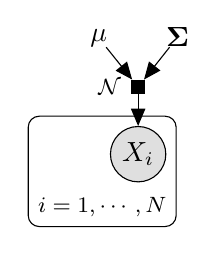
\begin{tikzpicture}
                
                
            \node[obs]                               (xn) {$X_i$};
            \factor[above=of xn] {y-f} {left:${\mathcal{N}}$} {} {} ; %
            \node[const, above=1 of xn, xshift=0.5cm] (sigma) {$\mathbf{\Sigma}$};
            \node[const, above=1 of xn, xshift=-0.5cm] (mu) {$\mathbf{\mathbf{\mu}}$};
            \plate{}{(xn)}{$i = 1, \cdots, N$};
            
            
            
            \edge {y-f} {xn} ; %
            \edge {mu, sigma} {y-f} ; %
            
            
        \end{tikzpicture}
\end{frame}
\begin{frame}
Let us assume we have a dataset $D = \{x_1, x_2, \ldots, x_n\}$, where each $x_i$ is an independent sample from the above distribution.
We want to estimate the parameters $\theta = {\mu, \sigma}$ from the data.

Our likelihood function is given by:
\begin{equation}
P(D|\theta) = \mathcal{L}(\mu, \Sigma) = \prod_{i=1}^n f(x_i|\mu, \Sigma)
\end{equation}

\end{frame}

\begin{frame}
    For example: A bivariate Normal distribution can be visualized as given below:
    \begin{figure}
                \centerline{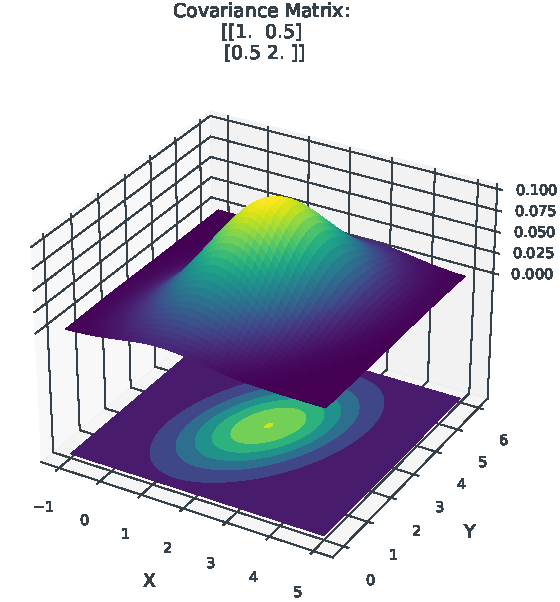
\includegraphics[scale = 0.75]{../figures/mle/bivariate_normal.pdf}}
\end{figure}
    
\end{frame}

\begin{frame}{Log Likelihood Function}
    Log-likelihood function:
    \begin{equation}
        \log \mathcal{L}(\mu, \Sigma) = \sum_{i=1}^n \log f(x_i|\mu, \Sigma)
    \end{equation}

    Simplifying the above equation, we get:
    \begin{align*}
        \log \mathcal{L}(\mu, \Sigma) &= \sum_{i=1}^n \log f(x_i|\mu, \Sigma) \\
        &= \sum_{i=1}^n \log \left((2\pi)^{-\frac{k}{2}}\det(\Sigma)^{-\frac{1}{2}}exp^{-\frac{1}{2}(x_i-\mu)^{T}\Sigma^{-1}(x_i-\mu)} \right) \\
        &= \sum_{i=1}^n \log ((2\pi)^{-\frac{k}{2}}) + \sum_{i=1}^n \log (\det(\Sigma)^{-\frac{1}{2}}) + \\ & \ \ \ \sum_{i=1}^n \log(exp^{-\frac{1}{2}(x_i-\mu)^{T}\Sigma^{-1}(x_i-\mu)} )) 
        \end{align*}
\end{frame}

\begin{frame}
    Continuing, we get:
    \begin{align*}
        = -\frac{kn}{2}\log(2\pi) -\frac{n}{2}\log(\Sigma) -\frac{1}{2}\sum_{i=1}^n (x_i-\mu)^T\Sigma^{-1}(x_i-\mu)  
        \end{align*}

    \begin{tcolorbox}[colback=metropolisblue!5,colframe=metropolisblue,title=Log Likelihood Function for Multivariate Normal Distribution]
            Log-likelihood function for multivariate normally distributed data is:
            \[
                -\frac{kn}{2}\log(2\pi) -\frac{n}{2}\log(\Sigma) -\frac{1}{2}\sum_{i=1}^n (x_i-\mu)^T\Sigma^{-1}(x_i-\mu)
                \]
        \end{tcolorbox}
\end{frame}

\begin{frame}
    \frametitle{Maximum Likelihood Estimate for $\mu$}
    
    To find the MLE for $\mu$, we differentiate the log-likelihood function with respect to $\mu$ and set it to zero:
    
    \begin{align*}
      &=\frac{\partial}{\partial \mu} \left(-\frac{kn}{2}\log(2\pi) -\frac{n}{2}\log(\Sigma) -\frac{1}{2}\sum_{i=1}^n (x_i-\mu)^T\Sigma^{-1}(x_i-\mu)\right) \\
      &= \frac{\partial}{\partial \mu} \left(-\frac{1}{2} \sum_{i=1}^n (x_i-\mu)^T\Sigma^{-1}(x_i-\mu)\right) \\
      &= -\frac{1}{2}\sum_{i=1}^n \left(\Sigma^{-1}(x_i-\mu) + (x_i-\mu)^T\Sigma^{-1} \right) = 0\\
      &= -\frac{1}{2} \sum_{i=1}^n 2\Sigma^{-1}(x_i-\mu) = 0 
    \end{align*} \centerline{as $(x_i-\mu)^{T}\Sigma^{-1} = \Sigma^{-1}(x_i-\mu)$}
    
\end{frame}

\begin{frame}
    
    \begin{align*}
      &=\Sigma^{-1}\sum_{i=1}^n(x_i-\mu) = 0 \\
      &=\sum_{i=1}^n(x_i) - n\mu = 0 \\
      &\mu = \frac{\sum_{i=1}^n x_i}{n}      
    \end{align*} 

    \begin{tcolorbox}[colback=metropolisblue!5,colframe=metropolisblue,title=Maximum Likelihood Estimate for $\mu$]
        MLE of $\mu$, denoted as $\hat{\mu}_{\text{MLE}}$, is given by:
        \begin{equation*}
            \hat{\mu}_{\text{MLE}} = \frac{1}{n}\sum_{i=1}^n x_i
        \end{equation*}
    \end{tcolorbox}
    
\end{frame}

\begin{frame}{MLE for $\Sigma$ for multivariate normally distributed data}
    Recall that the log-likelihood function is given by:
    \begin{equation}
        \log \mathcal{L}(\mu, \Sigma) = \sum_{i=1}^n \log f(x_i|\mu, \Sigma)
    \end{equation}

    Let us find the maximum likelihood estimate of $\Sigma$ now. We can do this by taking the derivative of the log-likelihood function with respect to $\Sigma$ and equating it to zero.   

    \begin{equation}
        \frac{\partial \log \mathcal{L}(\mu, \Sigma)}{\partial \Sigma} = \sum_{i=1}^n \frac{\partial \log f(x_i|\mu, \Sigma)}{\partial \Sigma} = 0
    \end{equation}
    
\end{frame}
\begin{frame}
    After differentiating and simplifying, we get:
    \begin{align*}
      \Sigma = \frac{1}{n}\sum_{i=1}^n(x_i-\mu)(x_i-\mu)^T  
    \end{align*} 

    \begin{tcolorbox}[colback=metropolisblue!5,colframe=metropolisblue,title=Maximum Likelihood Estimate for $\Sigma$]
        MLE of $\Sigma$, denoted as $\hat{\Sigma}_{\text{MLE}}$, is given by:
        \begin{equation*}
            \hat{\Sigma}_{\text{MLE}} = \frac{1}{n}\sum_{i=1}^n (x_i-\mu)(x_i-\mu)^T
        \end{equation*}
    \end{tcolorbox}
\end{frame}

\section{MLE for Linear Regression}
\begin{frame}{MLE for Linear Regression}
\begin{figure}
                \centerline{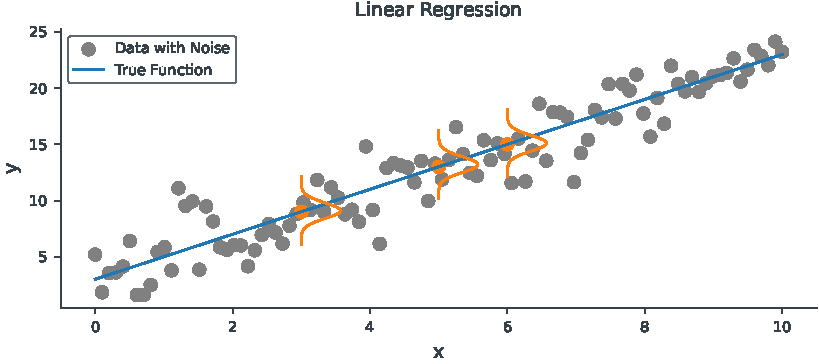
\includegraphics[scale=0.7]{../figures/mle/normal_likelihood_lin_reg.pdf}}
\end{figure}
We consider a regression problem with the likelihood function: $p(y|x) = \mathbb{N}(y|f(x), \sigma^2)$.\\
Let us assume we have a dataset $D = \{(x_1, y_1), (x_2,y_2), \ldots, (x_n, y_n)\}$, where $x_i\in R^d, y_i\in R$. 
\end{frame}

\begin{frame}
The functional relationship between $x$ and $y$ is given as $y = f(\bold{x})+\epsilon$ where $\epsilon\sim \mathbb{N}(0, \sigma^2).$ \\ 
Thus $f(\bold{x}) = x^T\theta.$\\ 
\addlinespace
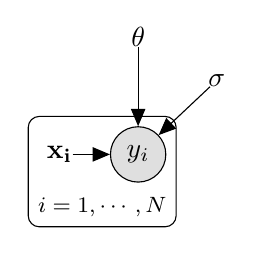
\begin{tikzpicture}
                
                
    \node[obs]                               (yi) {$y_i$};
    \node[const, xshift=-1cm](xi) {$\mathbf{x_i}$};
    \node[const, above=1 of yi](theta)
    {$\mathbf{\theta}$};
    \node[const, above=0.5 of yi, xshift=1cm](sigma)
    {$\mathbf{\sigma}$};
    \plate{}{(yi)}{$i = 1, \cdots, N$};
    \edge{theta}{yi}
    \edge{sigma}{yi}
    \edge{xi}{yi}
            
            
\end{tikzpicture}

\end{frame}


\begin{frame}
Our likelihood function (Normal distribution) is given by:
\begin{equation}
P(\mathcal{Y}|\mathcal{X},\theta) = p(y_1,\ldots,y_n|x_1,\ldots,x_n,\theta) = \prod_{i=1}^n p(y_i|x_i, \theta) 
\end{equation}

The MLE equation is given by:
\begin{equation}
    \theta_{MLE}\in \arg_{\theta} \max p(\emph{Y}|\emph{X},\theta)
\end{equation}
Maximizing the likelihood $\sim$ Maximizing the log likelihood $\sim$ Minimizing the negative log likelihood.\\
Taking negative log, we get:
    \begin{align*}
        -\log p(\mathcal{Y} \mid \mathcal{X}, \boldsymbol{\theta})&=-\log \prod_{i=1}^N p\left(y_i \mid \boldsymbol{x}_i, \boldsymbol{\theta}\right)=-\sum_{i=1}^N \log p\left(y_i \mid \boldsymbol{x}_i, \boldsymbol{\theta}\right)
    \end{align*}
    For a given point $(x_i, y_i),$
    \begin{align*}
         \log p\left(y_i \mid \boldsymbol{x}_i, \boldsymbol{\theta}\right)=-\frac{1}{2 \sigma^2}\left(y_i-\boldsymbol{x}_i^{\top} \boldsymbol{\theta}\right)^2+ const
    \end{align*}
\end{frame}

\begin{frame}
Thus the log likelihood is simplified to:
\begin{align*} \mathcal{L}(\boldsymbol{\theta}) & :=\frac{1}{2 \sigma^2} \sum_{n=1}^N\left(y_n-\boldsymbol{x}_n^{\top} \boldsymbol{\theta}\right)^2 \\ & =\frac{1}{2 \sigma^2}(\boldsymbol{y}-\boldsymbol{X} \boldsymbol{\theta})^{\top}(\boldsymbol{y}-\boldsymbol{X} \boldsymbol{\theta})=\frac{1}{2 \sigma^2}\|\boldsymbol{y}-\boldsymbol{X} \boldsymbol{\theta}\|^2\end{align*}\\
This is none other than squared error loss! To minimize this, we differentiate wrt $\theta$. In the end, we get:\\
    \begin{equation}
        \theta &= (X^TX)^{-1}X^Ty
    \end{equation}
    \begin{tcolorbox}[colback=metropolisblue!5,colframe=metropolisblue,title=Maximum Likelihood Estimate for $w$]
        MLE of $\theta$, denoted as $\hat{w}_{\text{MLE}}$, is given by:
        \begin{equation*}
            \hat{\theta}_{\text{MLE}} = (X^TX)^{-1}X^Ty
        \end{equation*}
    \end{tcolorbox}
\end{frame}


\section{MLE for Logistic Regression}

\begin{frame}{MLE for Logistic Regression}
% \begin{tikzpicture}
                
                
%     \node[obs]                               (y_i) {$x_i\theta$};
%     \node[const, xshift=-1cm](xi) {$\mathbf{x_i}$};
%     \node[const, above=1 of yi](theta){$\mathbf{\theta}$};
%     \node[const, xshift=1.5cm](pxi) {$p(x_i)$}
%     \node[const, xshift=2.5cm](beta) {$\beta$}
%     \plate{}{(yi)}{$i = 1, \cdots, N$};
%     \edge{yi}{pxi}
%     \edge{pxi}{beta}
%     \edge{theta}{yi}
%     \edge{xi}{yi}
            
            
% \end{tikzpicture}\\

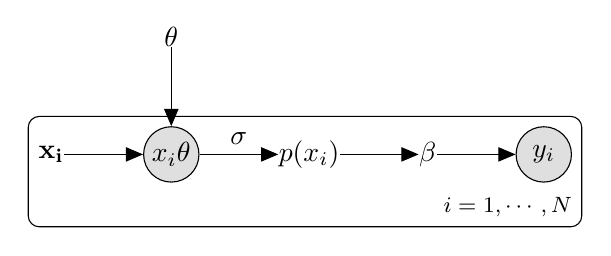
\begin{tikzpicture}

\node[obs] (x_i_theta) {$x_i\theta$};
\node[const, left=of x_i_theta] (xi) {$\mathbf{x_i}$};
\node[const, above=of x_i_theta] (theta) {$\mathbf{\theta}$};
\node[const, right=of x_i_theta] (pxi) {$p(x_i)$};
\node[const, right=of pxi] (beta) {$\beta$};
\node[obs, right=of beta] (yi_out) {$y_i$};
\plate {plate1} {(xi)(x_i_theta)(yi_out)} {$i = 1, \cdots, N$};

\draw[->] (xi) -- (x_i_theta);
\draw[->] (theta) -- (x_i_theta);
\draw[->] (x_i_theta) -- node[above] {$\sigma$} (pxi); % Adding "sigma" text
\draw[->] (pxi) -- (beta);
\draw[->] (beta) -- (yi_out);

\end{tikzpicture}






The probability distribution in case of Logistic Regression considering two classes is Bernoulli distribution but there is a slight difference. The probability is now the output of the logistic function.
Parameters are $\theta=[\beta_0,\beta_1]$.
\begin{equation}
p = P(Y=1|X) = \frac{1}{1+e^{-(\beta_0+\beta_1X)}}
\end{equation}


\end{frame}

\begin{frame}
Rewriting the likelihood in this manner:
\begin{align*}
    \mathbb{L}(\beta)&= \prod_{y_i=1}p(x_i)\prod_{y_i=0}(1-p(x_i))\\
    &=\prod\left(p(x_i)^{y_i}(1-p(x_i))^{1-y_i}\right)
\end{align*}
Taking log on both sides:\\
\begin{align*}
    L(\beta) &= \sum_{i=1}^n y_i\log(p(x_i)) + (1-y_i)\log(1-p(x_i))
\end{align*}
Substituting p from above equation. 
\begin{align}
    L(\beta) &= \sum_{i=1}^ny_i\log\left(\frac{1}{1+e^{-\beta x_i}}\right) + (1-y_i)\log\left(\frac{e^{-\beta x_i}}{1+e^{-\beta x_i}}\right)
\end{align}
\end{frame}

\begin{frame}
    Now if we differentiate this wrt $\beta$, it is difficult to find a analytical solution with it.
    Thus in order to solve for MLE for logistic regression, methods like Gradient Descent, Newton-Raphson, etc. are used. For example through Gradient descent, the below decision boundary i.e. $\beta$ has been calculated.
    \begin{figure}
                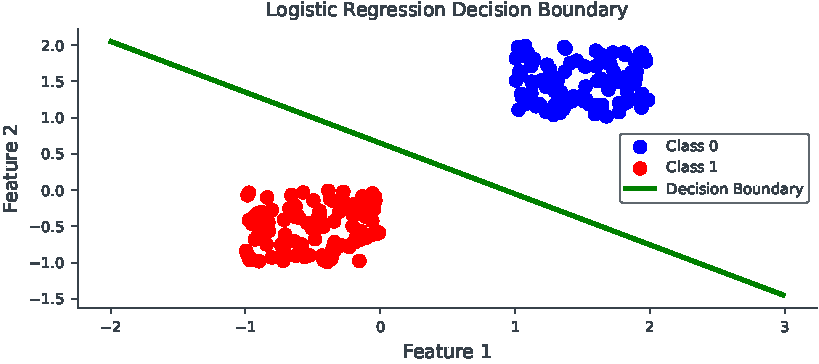
\includegraphics[scale=0.8]{../figures/mle/log_reg.pdf}
            \end{figure}
\end{frame}

    \begin{frame}{Random variable and Random sample}
    Random variable: $X:\Omega\rightarrow\mathbb{R}$ is a function from the sample space to the real line. \\ 
    \addlinespace
    \addlinespace
    Random sample: Collection of $n$ independent and identically distributed (i.i.d.) random variables $X_1, X_2, X_3, \ldots, X_n$. A group of experiments constitutes a sample.\\
    \addlinespace
    \addlinespace
    For example:\\
    Random variable: Y (possible outcomes 1 to 6)\\
    Random sample: {4,2,6} (outcomes of three consecutive die tosses)
    \end{frame}

    \begin{frame}{Bias of an Estimator}
        \begin{tcolorbox}[colback=metropolisblue!5,colframe=metropolisblue,title=Bias of an Estimator]
            The bias of an estimator $\hat{\theta}$ of a parameter $\theta$ is defined as:
            \[
                \text{Bias}(\hat{\theta}) = \mathbb{E}(\hat{\theta}) - \theta
            \]
            where $\mathbb{E}(\hat{\theta})$ is the expected value of the estimator $\hat{\theta}$.
        \end{tcolorbox}
        \begin{itemize}
            \item An estimator is said to be unbiased if $\text{Bias}(\hat{\theta}) = 0$.
            \item An estimator is said to be biased if $\text{Bias}(\hat{\theta}) \neq 0$.
        \end{itemize}
        
    \end{frame}
    

    \begin{frame}{Bias of an Estimator: $\hat{\mu}_{MLE}$}
        \pause 
        Question: What is the expectation of $\hat{\mu}_{MLE}$ calculated over? What is the source of randomness? \\
        If $X_i's$ are normally distributed random variables with mean $\mu$ and variance $\sigma^2 $ respectively, then $E(X_i) = \mu$ and $Var(X_i)=\sigma^2.$

        Recall that if an estimator $\hat{\theta}$ of a parameter $\theta$ is unbiased then:\\
        $\mathbb{E}(\hat{\theta})=\theta.$
    
        
    \end{frame}
    
    \begin{frame}{Bias of an Estimator: $\hat{\mu}_{MLE}$}
        
        \begin{align*}
            \mathbb{E}(\hat{\mu}_{MLE}) &= \mathbb{E}(\Bar{X}) \\
            &=\mathbb{E}\left(\frac{1}{n}\sum_{i=1}^nX_i\right) \\
            &=\frac{1}{n}\sum_{i=1}^n\mathbb{E}(X_i) \\
            &=\frac{1}{n}(n\mu) = \mu
        \end{align*}
        
        
        % Add tcolorbox here
        \begin{tcolorbox}[colback=metropolisblue!5,colframe=metropolisblue,title= Estimator $\hat{\mu}_{MLE}$ is unbiased]
            $\mathbb{E}(\hat{\mu}_{MLE}) = \mu$
        \end{tcolorbox}

        
    \end{frame}

    \begin{frame}
        \frametitle{Bias of $\sigma^2_{MLE}$}
        
        The MLE of $\sigma^2$ is given by
        
        $\hat{\sigma}^2_{MLE} = \frac{1}{n} \sum_{i=1}^n (x_i-\Bar{x})^2$.
        
        \begin{align*}
            \hat{\sigma}^2 &= \frac{1}{n} \sum_{i=1}^n (x_i-\Bar{x})^2 \\
            &= \frac{1}{n} \sum_{i=1}^n x_i^2 - 2\Bar{x} x_i + \Bar{x}^2 = \frac{1}{n} \sum_{i=1}^n x_i^2  -2\Bar{x}\frac{1}{n}\sum_{i=1}^nx_i+ \Bar{x}^2 \\
            &= \frac{1}{n}\sum_{i=1}^nx_i^2 - \Bar{x}^2
            \end{align*}

        \end{frame}

    \begin{frame}{Bias of $\sigma^2_{MLE}$}
        \begin{align*}
            \mathbb{E}(\hat{\sigma}^2) &=\mathbb{E}\left[\frac{1}{n}\sum_{i=1}^nX_i^2-\Bar{X}^2 \right] = \left[\frac{1}{n}\sum_{i=1}^n\mathbb{E}(X_i^2)\right]-\mathbb{E}(\Bar{X}^2)\\
            &=\frac{1}{n}\sum_{i=1}^n\left(\sigma^2+\mu^2\right) - \left(\frac{\sigma^2}{n}+\mu^2\right)\\
            &=\frac{1}{n}\left(n\sigma^2+n\mu^2\right) - \frac{\sigma^2}{n}-\mu^2\\
            &= \sigma^2 - \frac{\sigma^2}{n} = \frac{n\sigma^2-\sigma^2}{n} = \frac{(n-1)\sigma^2}{n}
        \end{align*}
        \begin{tcolorbox}[colback=metropolisblue!5,colframe=metropolisblue,title= Estimator $\hat{\sigma}_{MLE}$ is biased]
            $\mathbb{E}(\hat{\sigma}_{MLE}) = \frac{(n-1)\sigma^2}{n}$
        \end{tcolorbox}
    \end{frame}

        \begin{frame}{Bias }
            \begin{figure}
                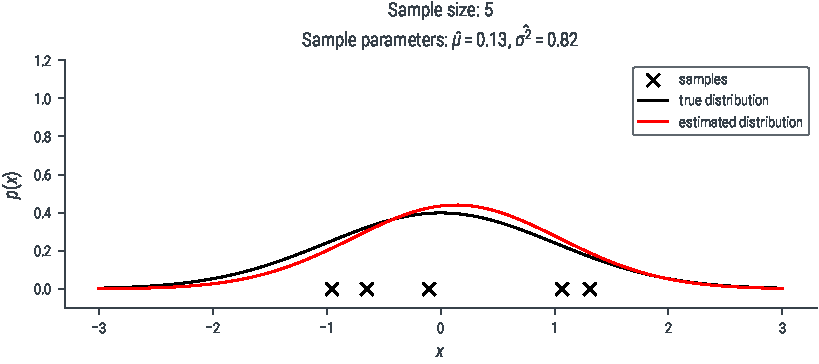
\includegraphics{../figures/mle/biased-mle-normal-5-0.pdf}
            \end{figure}
            
        \end{frame}

             \begin{frame}{Bias }
            \begin{figure}
                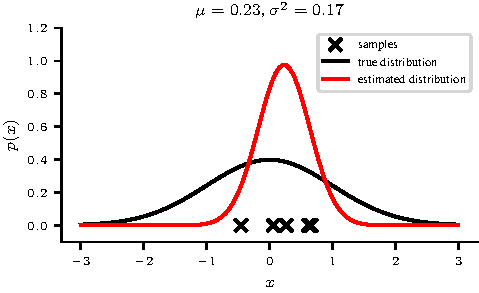
\includegraphics{../figures/mle/biased-mle-normal-5-1.pdf}
            \end{figure}
            
        \end{frame}

             \begin{frame}{Bias }
            \begin{figure}
                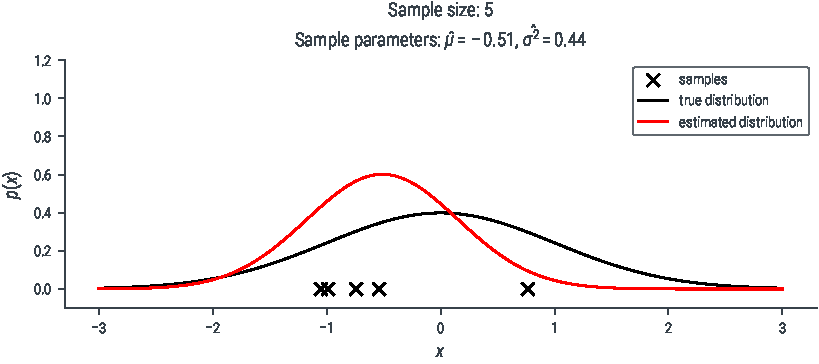
\includegraphics{../figures/mle/biased-mle-normal-5-2.pdf}
            \end{figure}
            
        \end{frame}

             \begin{frame}{Bias }
            \begin{figure}
                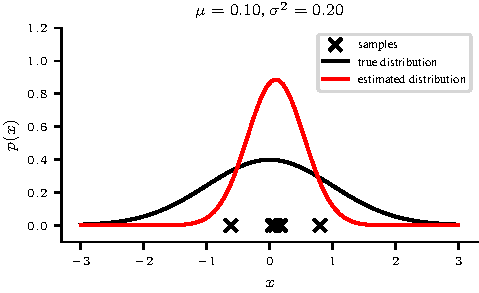
\includegraphics{../figures/mle/biased-mle-normal-5-3.pdf}
            \end{figure}
            
        \end{frame}

             \begin{frame}{Bias }
            \begin{figure}
                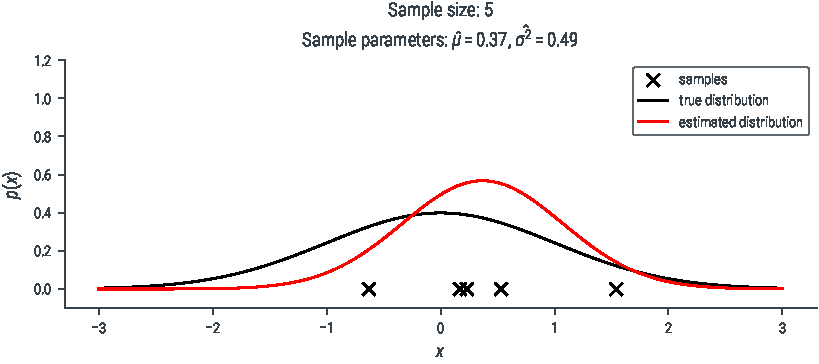
\includegraphics{../figures/mle/biased-mle-normal-5-4.pdf}
            \end{figure}
            
        \end{frame}

             \begin{frame}{Bias }
            \begin{figure}
                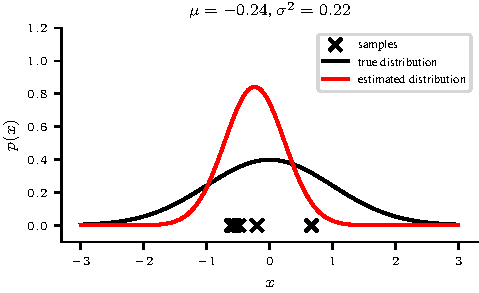
\includegraphics{../figures/mle/biased-mle-normal-5-5.pdf}
            \end{figure}
            
        \end{frame}

\begin{frame}{MAP Plate Notation for Beta-Bernoulli}
    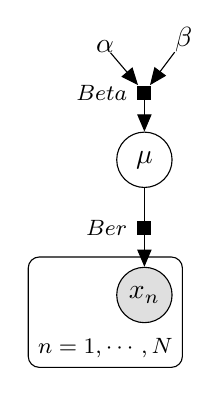
\begin{tikzpicture}
                
                
                \node[obs]                               (xn) {$x_n$};
                \node[latent, above=of xn] (mu) {$\mathbf{\mu}$};
                \factor[above=of xn] {y-f} {left:${Ber}$} {} {} ; %
                \node[const, above=1 of mu, xshift=0.5cm] (beta) {$\mathbf{\beta}$};
                \node[const, above=1 of mu, xshift=-0.5cm] (alpha) {$\mathbf{\alpha}$};
                \factor[above=of mu] {mu-f} {left:${Beta}$} {} {} ; %
                \plate{}{(xn)}{$n = 1, \cdots, N$};
                
                
                
                \edge {mu} {xn} ; %
                \edge {alpha,beta} {mu-f} ; %
                \edge  {mu-f}{mu} ; %
                
                
            \end{tikzpicture}
\end{frame}


    

    


    

\end{document}